\section{Installationsanleitung}

\subsection{DNA Center Setup}



\subsubsection{DNA Center Reset}
Da nach einigen Versuchen weder ein funktionsfähiges Under- noch Overlay Netzwerk vorhanden war, hatten wir uns entschieden das DNA Center neu zu Konfigurieren.

\begin{lstlisting}[language=bash]
$ maglev-config-wizard #DO NOT EXECUTE THIS COMMAND
\end{lstlisting}

Als folge dieses Befehls, nachdem alle Parameter eingegeben wurden, kam die folgende Meldung:

\begin{figure}[H]
	\centering
	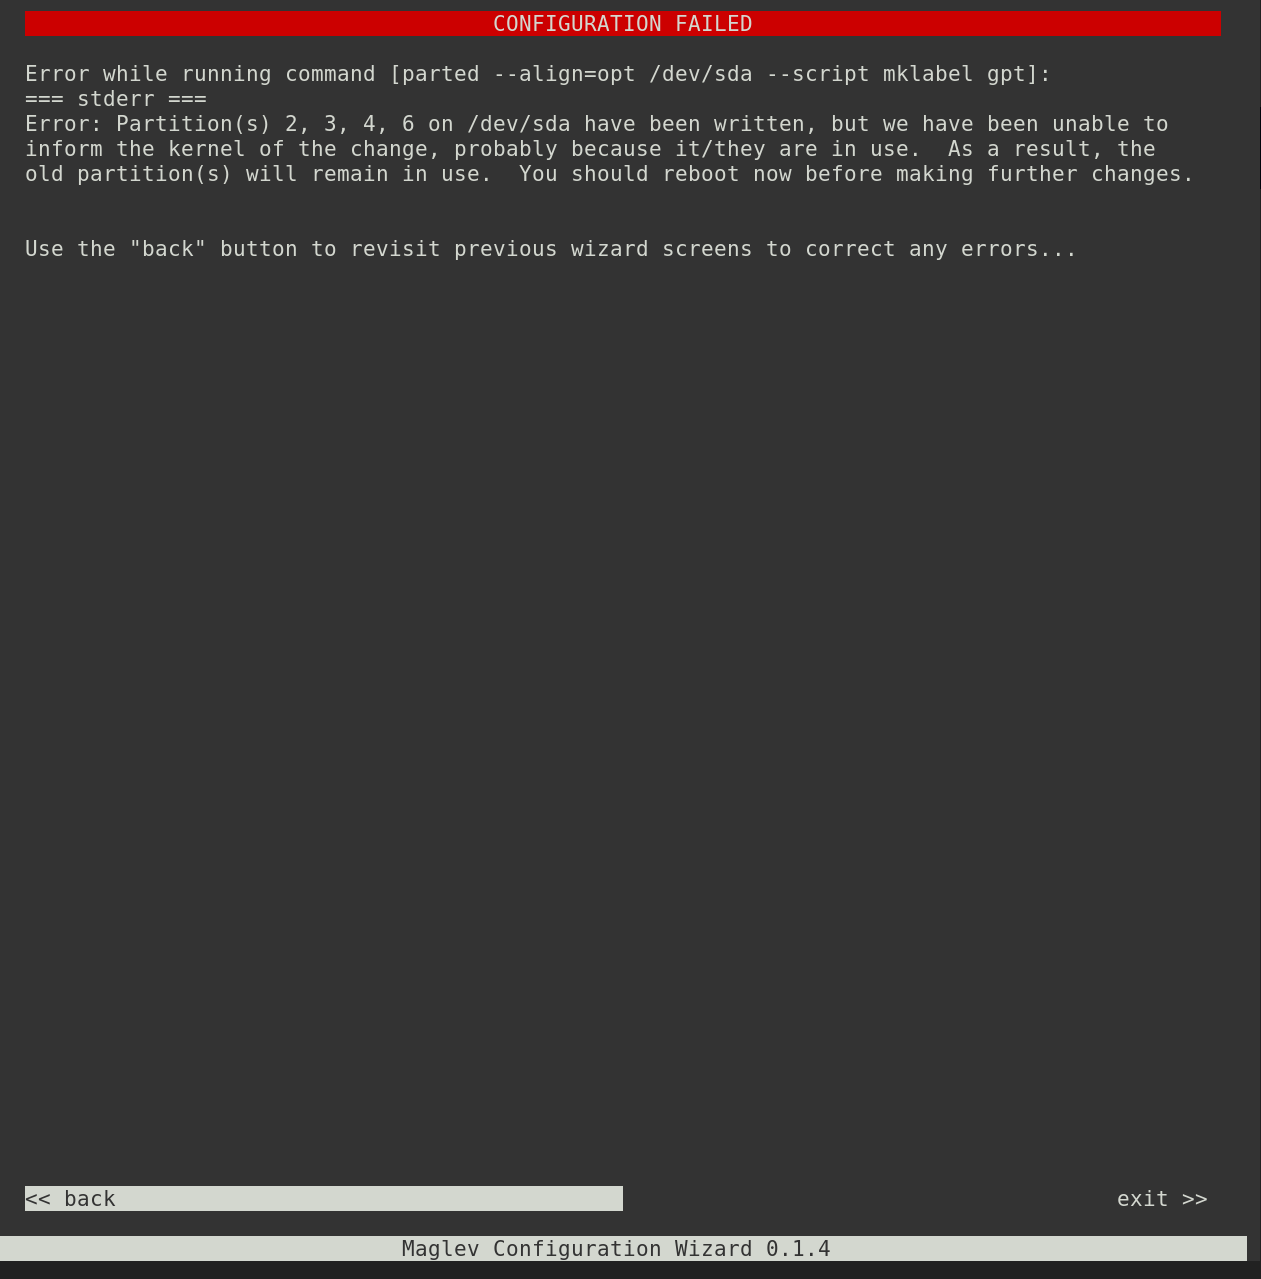
\includegraphics[height=10cm]{img/dna-center-reset-fail-1.png}
	\caption{DNA Center - maglev-config-wizard - Fehlermeldung}
	\label{fig:dna-center-reset-1}
\end{figure}

Nach einem Neustart der Appliance kam die folgende Meldung und das System bootete nicht mehr. 
\begin{figure}[H]
	\centering
	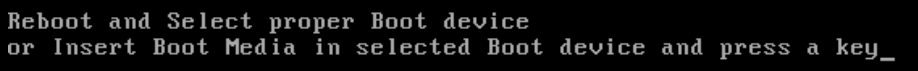
\includegraphics[height=1cm]{img/dna-center-reset-fail-2.png}
	\caption{DNA Center - Boot Fehlermeldung}
	\label{fig:dna-center-reset-2}
\end{figure}

In der Anleitung wird dieser Befehl so nicht erwähnt. Bei einem früheren Versuch diesen Befehl auszuführen, um den NTP Server zu ändern, führte es jedoch nicht zu diesem Fehler. 

\paragraph{Neuinstallation}
In folge war es notwendig die Cisco DNA Center Appliance neu zu installieren. 

\begin{figure}[H]
	\centering
	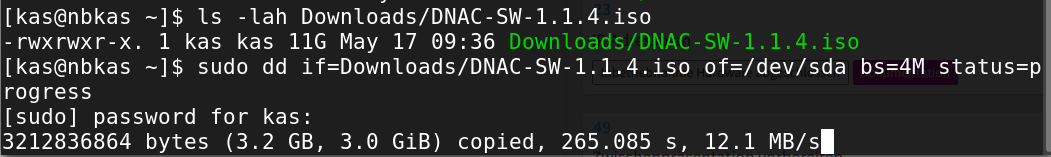
\includegraphics[height=2cm]{img/dna-center-reset-iso.png}
	\caption{DNA Center - Neuinstallation - Installations ISO wird auf USB Drive kopiert}
	\label{fig:dna-center-iso-1}
\end{figure}

Das USB Drive wird direkt in die Appliance gesteckt und gebootet. Der weitere Installationsprozess sieht aus wie im Abschnitt \ref{DNACenterSetup_Installation} gezeigt. 

\alertwarningbox{
	Nach der Neuinstallation sind alle Daten und die Konfiguration gelöscht. Eine Option die Konfiguration beizubehalten gibt es nicht.
}



\subsection{DNA Center Network Discovery}

Um die Netzwerkkomponenten zum DNA Center hinzuzufügen, wurde mehrere Versuche unternommen. 
